\section{概要}
本研究の実験フローを説明する.実験の概要を図\ref{fig:ml-flow}に示す.
これは予め用意されたデータセットと,検証内容に応じて設定された条件を入力として,精度を出力するまでの一連の流れである.\\

入力データとしては以下のものが設定されている.
\begin{description}
    \item [検証するデータセット] 30種類のデータセット(\ref{sec:dataset}節参照)
    \item [前処理] なし,標準化,正規化
    \item [オートエンコーダの構成] \mbox{}
        \begin{itemize}
            \item なし(オートエンコーダを使用しない)
            \item 各層の次元数:[データの特徴量数, 20, 10, 5, 10, 20, データの特徴量数]
            \item 各層の次元数:[データの特徴量数, 20, 15, 10, 5, 10, 15, 20, データの特徴量数]
            \item 各層の次元数:[データの特徴量数, 20, 15, 10, 15, 20, データの特徴量数]
        \end{itemize}
    \item [オートエンコーダの学習データ] 全てのデータ,多数派クラスのみ,少数派クラスのみ
    \item [AE特徴量の前処理] なし,標準化,正規化
    \item [ハイパーパラメータチューニング] なし,あり
    \item [機械学習モデル] \mbox{}
    \begin{itemize}
        \item ロジスティック回帰
        \item ランダムフォレスト
        \item サポートベクターマシン
        \item ニューラルネットワーク
        \item LightGBM
    \end{itemize} 
\end{description}

これらの入力を用いて,以下の流れで実験を行う.

\begin{enumerate}
  \item 実験に用いるデータセットの読み込み
  \item データセットを用いて,既存手法と提案手法の分類精度を比較する.
  \item 提案手法のパラメータを変更することで,分類精度にどのような影響があるかを調査する.
\end{enumerate}

\begin{figure}[htbp]  
  \centering
  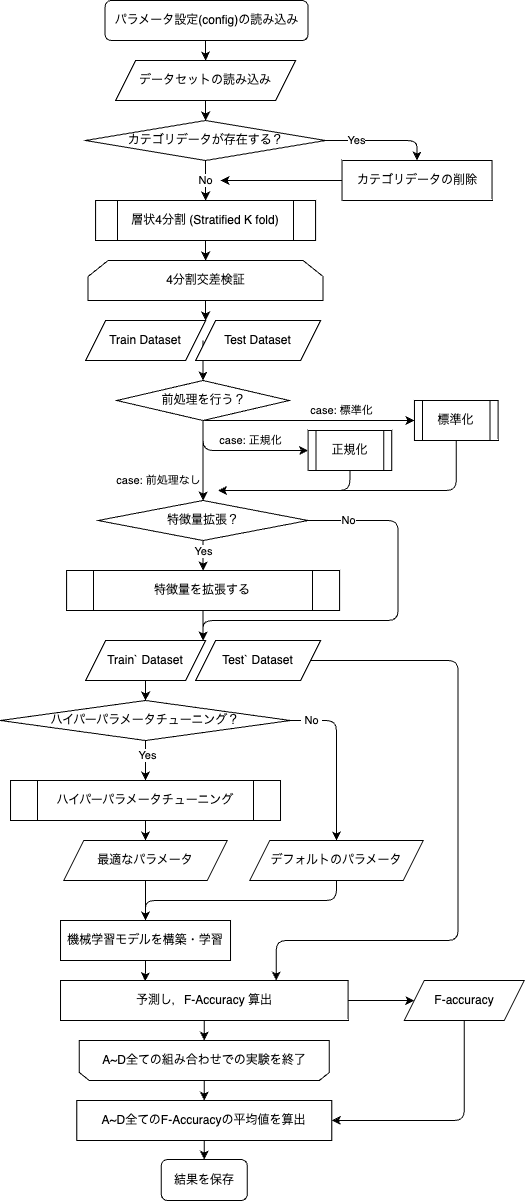
\includegraphics[width=0.6\linewidth\centering]{figures/ml-flow.png}
  \caption{実験の機械学習フロー}
  \label{fig:ml-flow}
\end{figure}
